\section{Introduction} \label{sec:intro}

% lineeaari tv -> videonauhuri -> on demand -> on demand tv
Before videocassette recorders became widely available for regular households, watching television was a very time-sensitive activity: if you wanted to see a TV program you had to watch it when it was broadcasted. When video recorders became affordable, they enabled people to record and watch TV programs whenever they wanted. Nowadays linear TV is losing even more of its foothold, as various video-on-demand services are gaining popularity. % at the expense of broadcast TV.
Recording storage is also moving away from the homes of viewers into the cloud servers of content providers.

% NVPR = videonauhuri pilvessä, jonka katsoja jakaa muiden kanssa
Network personal video recorder (NPVR) is a type of service for recording broadcast TV programs for later viewing. Instead of storing recordings on the users local device, NPVR stores recordings on the content providers server. For every program listed in the Electronic program guide (EPG), a single recording is created and stored on the server. The users who record the same program will receive the same video from the server.

% NPVR ongelma
The NPVR recording start and end times are determined by the scheduling information given in the EPG. However, it is common that programs are not broadcasted exactly according to the EPG schedule. To make sure that the whole program is recorded, some margin is typically added on both ends of the recording. Thus NPVR recordings tend to have some non-program content at the beginning and end. The goal of this thesis is to study whether user viewing behaviour can be used in determining where the closing credits begin in a NPVR recording.

% motivaatio
I am writing this thesis for a  NPVR service provider company. From the perspective of a NPVR service provider, closing credits detection has a few uses. Firstly, less storage space is needed if the surplus contet after the closing credits is discarded. Secondly, when the customers want to watch multiple episodes of a series in a row, it is convenient for them if a link to the next episode is displayed during the closing credits.

% rajaus
% User viewing behaviour might also be useful for detecting starting credits and advertisement breaks, but on this thesis I will focus on the closing credits detection to narrow down the topic. I will also restrict the examined recordings to TV series with multiple episodes and at least one hundred views per episode.

% sisältö ja rakenne
The main goal of this thesis is to study whether user viewing behaviour can be used for detecting closing credits of NPVR recordings. To support the empirical research, the theoretical background section discusses signal change detection, and result evaluation and validation. The empirical research section is divided into four parts. The ground truth is defined in the first part. The second part discusses the properties of the user viewing behaviour data. In the third part the Python scientific library Ruptures is used to detect closing credits. The results are evaluated in the fourth part. The discussion section considers, based on the previous sections, the viability of using user viewing behaviour for closing credits detection. Lastly, the main points of this thesis are summarised in the conclusions.

\section{Theoretical background} \label{sec:background}

\subsection{Signal change detection} \label{subsec:methods}

\subsection{Result evaluation and validation} \label{subsec:validation}

\section{Empirical research} \label{sec:casestudy}

\subsection{Ground truth} \label{subsec:groundtruth}

In order to evaluate how well a method detects NVPR closing credits, a ground truth is needed for comparison. The ground truth is obtained by direct human visual observation, meaning that a person must look at a video recording and write down the timestamps where the closing credits begin and end.

I have collected the closing credits start and end time from 510 NPVR recordings by hand with a margin of error of $\pm$ 1 seconds. Each of these recordings has at least one hundred user views.

\begin{figure}[H]
    \centering
    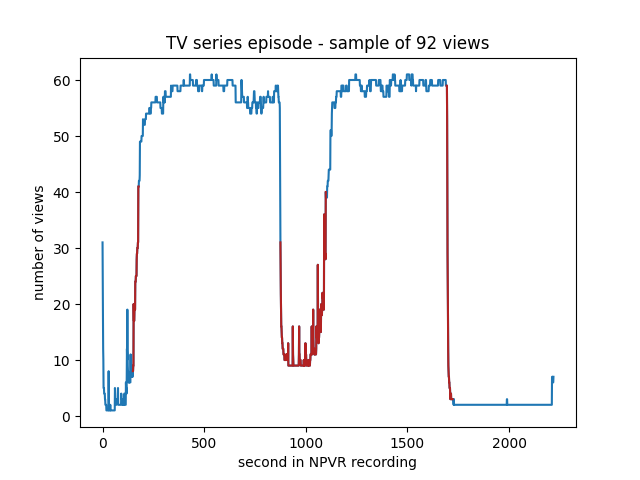
\includegraphics[width=1\textwidth]{../plots/episode.png}
    \caption{Visualisation of user views count for each second in an example NVPR recording}
    \label{fig:intro_ads_outro}
    \end{figure}

\subsection{User viewing behaviour data} \label{subsec:data}

Plotted in Figure \ref{fig:intro_ads_outro} is a sample of 92 user views of a NPVR recording. The horisontal axis contains one second long intervals, corresponding to every second of the recording. The vertical axis shows how many times a second long interval in the recording was viewed by users. For example, 58 users from the sample of 92 users watched the part of the video between 0:10:00 - 0:10:01 (600 on the horisontal axis in Figure \ref{fig:intro_ads_outro}).

The red colored part of the plot in Figure \ref{fig:intro_ads_outro} is where the starting credits, advertisement break and closing credits of the program are. I checked the location of the aforementioned by looking at the recorded video. A steep increase in views can be seen in the plot whenever the actual program content begins, and correspondingly there is a steep decrease in views when the program content shifts into to advertisements or closing credits.

\subsection{Closing credits detection with Ruptures library} \label{subsec:solution}

I will be using a Python library called Ruptures for the change point detection. Ruptures is based on the findings of a literature reviw conducted by Truong et al. \cite{truongSelectiveReviewOffline2020} which examines various methods for offline change point detection.

An example of Ruptures output is visualised on Figure \ref{fig:ruptures_change_detection}. The input data is the same as in Figure \ref{fig:intro_ads_outro}. Red rectangles on the plot represent the actual location of the starting credits, advertisement break and closing credits, respectively. The vertical dashed lines indicate the change points determined by Rupture. They appear to be very close to the genuine change points at the edges of the red blocks.

\begin{figure}[H]
\centering
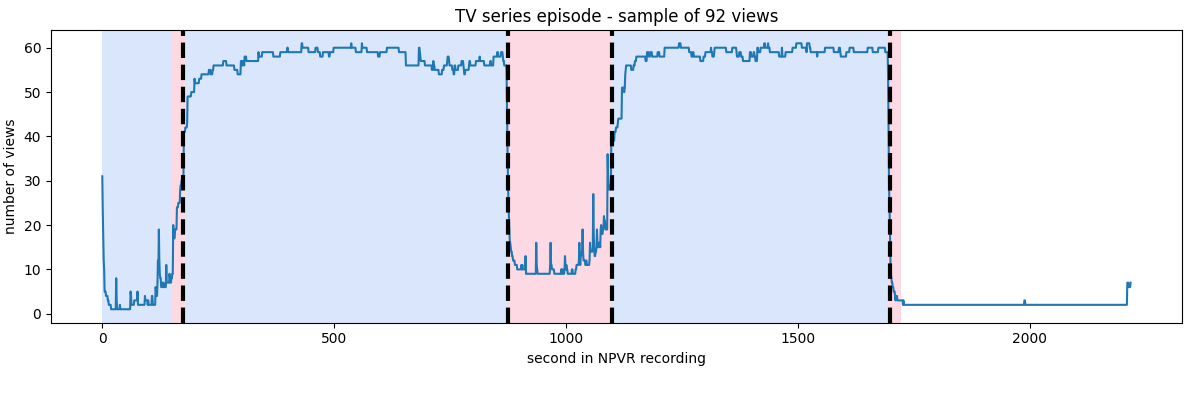
\includegraphics[width=1\textwidth]{../plots/episode-pen100.png}
\caption{Ruptures output for Figure \ref{fig:intro_ads_outro} data}
\label{fig:ruptures_change_detection}
\end{figure}

\subsection{Results} \label{sec:results}

\section{Discussion} \label{sec:discussion}

\section{Conclusions} \label{sec:conclusions}
